% ===========================================================================
% OpenDiscoveryTrace: Process Traces for Evaluating AI Scientist Workflows
% Submitted to the AI for Science workshop (ICML 2026)
% Dataset Competition Track
% ===========================================================================
\documentclass{article}
\usepackage{icml2026}

% Packages
\usepackage[T1]{fontenc}
\usepackage{amsmath,amssymb}
\usepackage{graphicx}
\usepackage{booktabs}
\usepackage{hyperref}
\usepackage{url}
\usepackage{xcolor}
\usepackage{listings}
\usepackage{multirow}
\usepackage{xspace}
\usepackage{microtype}

% Listings style for JSON
\lstdefinestyle{json}{
  basicstyle=\ttfamily\scriptsize,
  breaklines=true,
  frame=single,
  columns=fullflexible,
  showstringspaces=false,
  commentstyle=\color{gray},
  keywordstyle=\color{blue},
  stringstyle=\color{red!60!black},
  numbers=none,
  xleftmargin=2em,
  framexleftmargin=1.5em,
}

% Custom commands
\newcommand{\dataset}{\textsc{OpenDiscoveryTrace}\xspace}

\icmltitlerunning{OpenDiscoveryTrace}

\begin{document}

\twocolumn[
\icmltitle{OpenDiscoveryTrace: Process Traces for Evaluating\\AI Scientist Workflows}

\icmlsetsymbol{equal}{*}

\begin{icmlauthorlist}
\icmlauthor{Anonymous Author(s)}{anon}
\end{icmlauthorlist}

\icmlaffiliation{anon}{Under Review}

\icmlcorrespondingauthor{Anonymous Author(s)}{anon@example.com}

\icmlkeywords{AI for science, dataset, scientific agents, process evaluation, trajectory analysis}

\vskip 0.3in

\begin{abstract}
We propose \dataset, a dataset of 522 AI scientific agent trajectories capturing \emph{how} models reason through scientific tasks---not just what they produce. Each trajectory records a 9-field-per-step trace (thoughts, tool calls, errors, revisions, confidence) across 124 tasks in four science domains, executed by three frontier models and four open-weight models (7 total). Pilot analysis shows all models achieve similar success rates (${\sim}69\%$) yet differ dramatically in error profiles: Claude Opus 4.6 produces $30{\times}$ more errors than GPT-5.4, predominantly tool misuse (66.7\%) versus reasoning errors (83.6\%)---a dimension invisible to output-only benchmarks. We release the dataset, schema, harness, and five benchmark tasks under CC-BY-4.0.\footnote{Submitted to the AI for Science workshop (ICML 2026).}
\end{abstract}
]

\printAffiliationsAndNotice{}

% ===========================================================================
% SECTION 1: Scientific Bottleneck
% ===========================================================================
\section{Scientific Bottleneck}
\label{sec:bottleneck}

AI systems now conduct scientific research at scale: AlphaFold predicts protein structures at atomic accuracy~\citep{jumper2021alphafold}, GNoME discovers millions of stable crystals~\citep{merchant2023gnome}, and A-Lab synthesizes novel compounds autonomously~\citep{szymanski2023alab}. LLM-based agents have extended this to full research pipelines, generating hypotheses, running experiments, and producing papers~\citep{lu2024aiscientist,boiko2023coscientist,ghareeb2025robin}. An ecosystem of benchmarks has emerged to evaluate these systems~\citep{chen2025scienceagentbench,majumder2024discoverybench,starace2025paperbench,tian2024scicode,huang2024mlagentbench,chan2024mlebench,siegel2024corebench}, yet every existing benchmark evaluates only final outputs: generated code, terminal hypotheses, or rubric scores on replicated papers. The reasoning process is discarded entirely.

This creates three concrete problems for the field. First, the scientific method is fundamentally a process. Evaluating only outputs conflates reasoning quality with outcome luck: a model that systematically tests hypotheses and recovers from errors is scored identically to one that guesses correctly on its first attempt. Second, governance and auditing of AI scientists require complete decision traces to determine whether conclusions were reached through sound methodology~\citep{kapoor2023leakage,hung2024levels}. As autonomous science systems move toward deployment in safety-critical domains~\citep{tom2024selfdriving,abolhasani2023selfdriving}, the ability to audit the full reasoning chain becomes a prerequisite, not a luxury. Third, improving AI scientific agents requires understanding their failure modes, which are properties of trajectories, not of final answers. Without process data, we cannot distinguish between agents that need better tool interfaces and those that need better reasoning capabilities.

\dataset addresses this bottleneck by providing the first public dataset of complete, structured AI scientific agent process traces with error logging, revision tracking, and multi-phase workflow annotation.

% ===========================================================================
% SECTION 2: Proposed Dataset
% ===========================================================================
\section{Proposed Dataset}
\label{sec:dataset}

\dataset comprises 372 frontier-model trajectories spanning 124 tasks across four scientific domains (drug discovery, materials science, genomics, scientific literature) at three difficulty levels. Three frontier models (GPT-5.4, Claude Opus 4.6, Gemini 3.1 Pro) each execute all 124 tasks, yielding a fully balanced design (31 tasks per model per domain). The dataset additionally includes \textbf{120 open-weight model trajectories} from four models---Qwen2.5-7B-Instruct, Mistral-7B-Instruct-v0.3, Phi-3.5-mini-instruct, and Qwen2.5-1.5B-Instruct (30 tasks each)---enabling fully reproducible baselines without proprietary API access. Plus 30 live-retrieval variant trajectories. In total: \textbf{522 trajectories across 7 models}.

Each trajectory step records nine fields extending the ReAct format~\citep{yao2023react}: \texttt{step\_id}, \texttt{timestamp}, \texttt{phase} (literature review, hypothesis, experiment design, execution, analysis, revision, or conclusion), \texttt{thought}, \texttt{action} (tool, input, output), \texttt{observation}, \texttt{error} (type and message), \texttt{revision\_trigger}, and \texttt{confidence}. Outcome metadata includes success, final claim, verification result, failure type, and recovery status. The complete JSON schema is in Appendix~\ref{app:schema}.

Five benchmark tasks are defined on this data: (1)~trajectory outcome prediction, (2)~error localization, (3)~claim verification, (4)~autonomy level classification~\citep{tom2024selfdriving,hung2024levels}, and (5)~process quality scoring.

\begin{figure}[t]
    \centering
    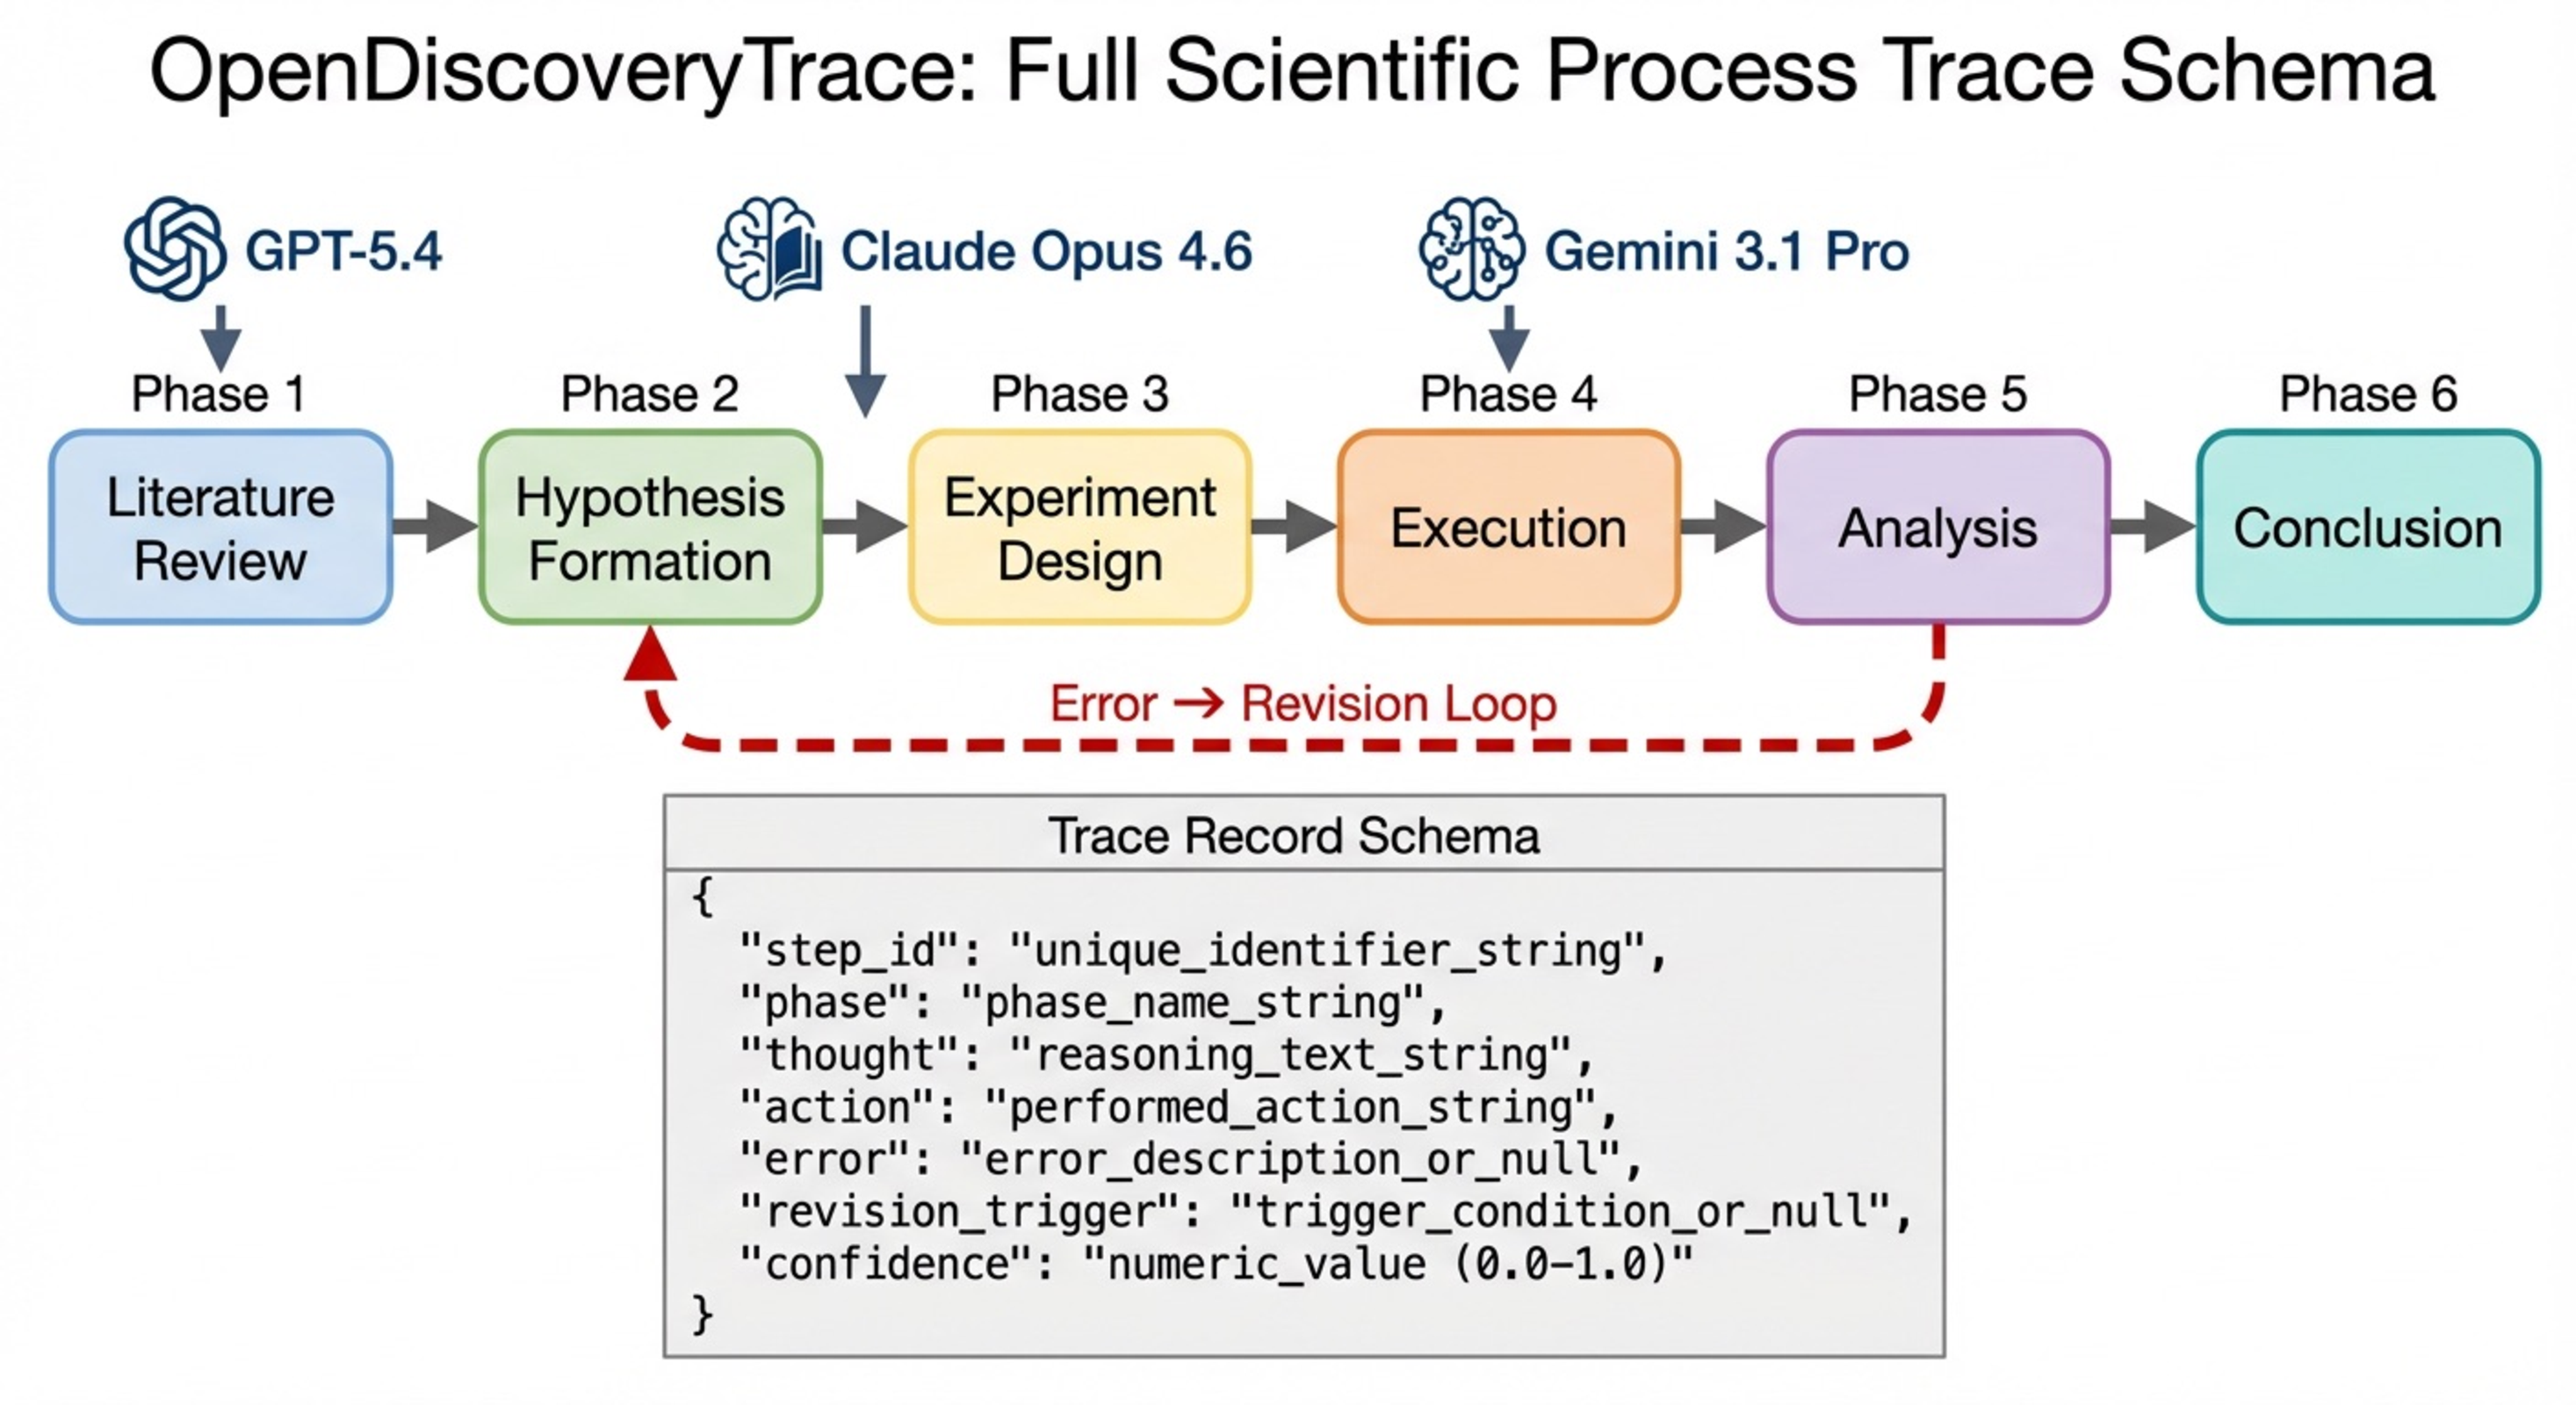
\includegraphics[width=\columnwidth]{figures/fig_architecture.pdf}
    \vspace{-1.5em}
    \caption{\footnotesize \textbf{\dataset architecture.} Seven models (3 frontier + 4 open-weight) execute tasks through a six-phase scientific workflow. Each step is logged as a 9-field trace. Failed steps trigger error-revision loops (dashed). The 522 trajectories form a structured corpus of AI scientific process traces.}
    \label{fig:architecture}
    \vspace{-1em}
\end{figure}

\textbf{Pilot evidence that process traces matter.} All three models achieve indistinguishable success rates (${\sim}69\%$, $p{=}0.997$) and step counts ($3.5{\pm}3.5$, $4.1{\pm}4.0$, $4.8{\pm}5.4$; $p{=}0.158$). However, error counts diverge dramatically: Claude Opus 4.6 averages $2.5{\pm}3.4$ errors per trajectory versus $0.08{\pm}0.3$ for GPT-5.4 (Kruskal-Wallis $H{=}122.0$, $p{<}0.0001$; Cliff's $\delta{=}0.613$, large). A failure taxonomy reveals qualitatively different error profiles: Claude's errors are 66.7\% tool misuse, GPT-5.4's are 83.6\% reasoning errors, and Gemini's are 72.1\% reasoning errors. Process traces expose this dimension; output-only benchmarks cannot. LSTM and Transformer baselines on trajectory outcome prediction match the majority baseline (Acc=0.693, AUROC${\leq}$0.422), confirming the task is non-trivial and motivating richer representations.

% ===========================================================================
% SECTION 3: Acquisition Roadmap
% ===========================================================================
\section{Acquisition Roadmap}
\label{sec:roadmap}

\textbf{Phase~1 (current).} 522 trajectories across 7 models (3~frontier + 4~open-weight), 124 tasks, 4 domains. Schema, harness, and benchmark tasks complete. 30 live-retrieval variant trajectories collected. Estimated cost: ${\sim}$\$300 API + ${\sim}$\$40 Modal GPU. All infrastructure is operational.

\textbf{Phase~2 (months 1--2).} Complete all 200 tasks across all 7 models. Add Llama~3.1-8B and Gemma-2-9B. Target: 1,800+ trajectories across 9 models, enabling robust cross-architecture comparisons between open-weight and frontier models on the full task bank.

\textbf{Phase~3 (months 2--3).} Human expert annotation on a 120-trajectory stratified sample. Three annotators score five axes (correctness, reasoning quality, tool use, autonomy level, error localization). Target: Krippendorff's $\alpha \geq 0.67$. LLM-based pilot already achieves $\alpha{=}0.63$--$0.82$ across axes, suggesting human agreement is attainable.

\textbf{Phase~4 (months 3--6).} Live retrieval integration for all literature-domain tasks via PubMed and PubChem APIs. Pilot ELN integration for physical-lab trace capture, extending the dataset from computational-only to hybrid computational-physical settings~\citep{dirnagl2016eln,abolhasani2023selfdriving}.

\textbf{Sustainability.} The schema is versioned with semver (v1.0 = current release). The dataset is hosted on HuggingFace with a DOI for citability. Annual refresh cycles incorporate new frontier models and expanded task banks. The harness is open-source, enabling community-contributed trajectories.

% ===========================================================================
% SECTION 4: Metadata, Governance & Safety
% ===========================================================================
\section{Metadata, Governance \& Safety}
\label{sec:governance}

\textbf{License and format.} CC-BY-4.0. Each trajectory is a self-contained JSON document following the 9-field schema (Appendix~\ref{app:schema}), with per-step and aggregate metadata. A datasheet following \citet{gebru2021datasheets} accompanies the release.

\textbf{Release tiers.} (1)~Full traces where provider terms of service permit redistribution. (2)~Abstracted state summaries (phase transitions, tool calls, error events without verbatim reasoning) where full release is restricted. Abstracted summaries preserve $>$90\% of analytical utility for error localization, process quality scoring, and autonomy classification.

\textbf{Privacy and safety.} No PII is present; all tasks use publicly available scientific knowledge. No wet-lab protocols or hazardous procedures are included. Tasks are sourced from established databases (ChEMBL, Materials Project, UniProt, KEGG).

\textbf{Versioning and splits.} Semver versioning with changelog. Task-level 80/20 train/test split with domain stratification ensures no data leakage across splits~\citep{kapoor2023leakage}. Evaluation methodology follows HELM~\citep{liang2023helm} for multi-faceted assessment.

\textbf{Provider policy.} We are working with each provider on release terms. The two-tier release strategy ensures the dataset remains useful even under restrictive redistribution policies.

% ===========================================================================
% SECTION 5: Acceleration Potential
% ===========================================================================
\section{Acceleration Potential}
\label{sec:acceleration}

\dataset enables six capabilities currently unavailable to the AI-for-science community. (1)~\emph{Process-aware agent evaluation}: benchmarking that distinguishes systematic reasoning from lucky guessing, complementing output-only metrics~\citep{wang2023scientific,gil2014amplify}. (2)~\emph{Early failure intervention}: 68.1\% of first errors occur at step~0, suggesting that monitoring initial tool invocations could prevent the majority of downstream failures. (3)~\emph{Error-type-specific training}: the discovery that Claude's errors are predominantly tool misuse while GPT-5.4's are reasoning errors implies different improvement strategies for each architecture. (4)~\emph{Process-aware reward modeling}: reward shaping over trajectories rather than outcomes, enabling RL approaches to agent training that credit good methodology independent of result. (5)~\emph{Trustworthy AI scientist auditing}: complete decision traces for governance of autonomous research systems~\citep{king2009automation,kitano2021nobel}. (6)~\emph{Reproducible open-weight benchmarking}: 120 trajectories from 4 open-weight models (Qwen2.5-7B, Mistral-7B, Phi-3.5-mini, Qwen2.5-1.5B) enable fully reproducible comparison without proprietary API keys, bridging the open/closed evaluation gap.

\dataset enables the shift from evaluating what AI scientists produce to evaluating how they reason, a prerequisite for trustworthy autonomous science.

% ===========================================================================
% REFERENCES
% ===========================================================================
\bibliography{references}
\bibliographystyle{icml2026}

% ===========================================================================
% APPENDIX
% ===========================================================================
\clearpage
\onecolumn
\appendix
\section*{Appendix}
\setcounter{section}{0}
\renewcommand{\thesection}{\Alph{section}}

\section{Full Trace Schema}
\label{app:schema}

Listing~\ref{lst:schema} shows the complete JSON schema for a single trajectory in \dataset.

\begin{lstlisting}[style=json, caption={Complete \dataset trace schema.}, label=lst:schema]
{
  "task_id": "string",
  "domain": "drug_discovery | materials_science
             | genomics | literature",
  "difficulty": "easy | medium | hard",
  "prompt": "string",
  "ground_truth": "string | null",
  "model": "gpt-5.4 | claude-opus-4-6
            | gemini-3.1-pro-preview",
  "trajectory": [
    {
      "step_id": "integer",
      "timestamp": "ISO8601",
      "phase": "literature_review | hypothesis
        | experiment_design | execution
        | analysis | revision | conclusion",
      "thought": "string",
      "action": {
        "type": "string",
        "tool": "string",
        "input": {},
        "output": {}
      },
      "observation": "string",
      "error": {
        "occurred": "boolean",
        "type": "string",
        "message": "string"
      },
      "revision_trigger": "string | null",
      "confidence": "float [0, 1]"
    }
  ],
  "outcome": {
    "success": "boolean",
    "final_claim": "string",
    "verification": {
      "method": "string",
      "result": "string",
      "score": "float"
    },
    "failure_type": "string | null",
    "recovery_attempted": "boolean"
  },
  "metadata": {
    "total_steps": "integer",
    "total_tokens": "integer",
    "total_tool_calls": "integer",
    "total_failures": "integer",
    "total_revisions": "integer",
    "wall_time_seconds": "float"
  }
}
\end{lstlisting}

\section{Benchmark Comparison}
\label{app:comparison}

% Comparison table: OpenDiscoveryTrace vs existing benchmarks
\begin{table*}[t]
\caption{Comparison of \dataset with existing AI science benchmarks. \dataset is the first benchmark to capture full process traces including error logging, revision tracking, and failure analysis alongside final output evaluation. $\checkmark$ = supported, $\times$ = not supported, $\sim$ = partial support.}
\label{tab:comparison}
\centering
\small
\begin{tabular}{lcccccc}
\toprule
\textbf{Benchmark} & \textbf{Process} & \textbf{Error} & \textbf{Revision} & \textbf{Multi-} & \textbf{Science} & \textbf{Multi-} \\
 & \textbf{Traces} & \textbf{Logging} & \textbf{Tracking} & \textbf{Domain} & \textbf{Specific} & \textbf{Model} \\
\midrule
ScienceAgentBench \citep{chen2025scienceagentbench} & $\times$ & $\times$ & $\times$ & $\checkmark$ & $\checkmark$ & $\checkmark$ \\
DiscoveryBench \citep{majumder2024discoverybench} & $\times$ & $\times$ & $\times$ & $\checkmark$ & $\checkmark$ & $\checkmark$ \\
The AI Scientist \citep{lu2024aiscientist} & $\times$ & $\times$ & $\times$ & $\sim$ & $\checkmark$ & $\checkmark$ \\
PaperBench \citep{starace2025paperbench} & $\times$ & $\times$ & $\times$ & $\sim$ & $\checkmark$ & $\checkmark$ \\
ResearchBench \citep{liu2025researchbench} & $\times$ & $\times$ & $\times$ & $\checkmark$ & $\checkmark$ & $\checkmark$ \\
SciCode \citep{tian2024scicode} & $\times$ & $\times$ & $\times$ & $\checkmark$ & $\checkmark$ & $\checkmark$ \\
MLAgentBench \citep{huang2024mlagentbench} & $\sim$ & $\sim$ & $\times$ & $\times$ & $\sim$ & $\checkmark$ \\
MLE-bench \citep{chan2024mlebench} & $\times$ & $\times$ & $\times$ & $\times$ & $\times$ & $\checkmark$ \\
WebArena \citep{zhou2024webarena} & $\checkmark$ & $\sim$ & $\times$ & $\times$ & $\times$ & $\checkmark$ \\
AgentBench \citep{liu2024agentbench} & $\checkmark$ & $\sim$ & $\times$ & $\times$ & $\times$ & $\checkmark$ \\
\midrule
\textbf{\dataset (ours)} & $\checkmark$ & $\checkmark$ & $\checkmark$ & $\checkmark$ & $\checkmark$ & $\checkmark$ \\
\bottomrule
\end{tabular}
\end{table*}


Table~\ref{tab:comparison} compares \dataset with existing AI science benchmarks. \dataset is the first to provide full process traces with error logging, revision tracking, and failure analysis alongside final output evaluation.

\section{Pilot Analysis Details}
\label{app:pilot}

\subsection{Dataset Statistics}

The current release comprises 522 trajectories: 372 from three frontier models (GPT-5.4, Claude Opus 4.6, Gemini 3.1 Pro; 124 each) with balanced domain coverage (31 per model per domain), plus 120 from four open-weight models (Qwen2.5-7B, Mistral-7B-v0.3, Phi-3.5-mini, Qwen2.5-1.5B; 30 each) and 30 live-retrieval variants. Among frontier trajectories, 99.7\% reach a conclusion. 31.2\% contain at least one error and 34.4\% contain at least one revision.

\begin{table}[h]
\caption{Dataset summary statistics.}
\label{tab:stats}
\centering
\small
\begin{tabular}{lc}
\toprule
\textbf{Metric} & \textbf{Value} \\
\midrule
Total trajectories & 522 \\
Models represented & 7 (3 frontier + 4 open-weight) \\
Domains covered & 4 \\
Tasks executed (per model) & 124 \\
Tasks designed (bank) & 200 \\
Conclusion rate & 99.7\% \\
Success rate (evaluable, $n{=}127$) & 69.3\% \\
Estimated total tokens & ${\sim}$701K \\
\midrule
Steps per trajectory (mean) & 4.1 \\
Tool calls per trajectory & 3.0 \\
Failures per trajectory & 1.0 \\
Revisions per trajectory & 0.87 \\
Wall time (seconds, mean) & 99.1 \\
\midrule
Trajectories with errors & 31.2\% \\
Trajectories with revisions & 34.4\% \\
\bottomrule
\end{tabular}
\end{table}

\subsection{Inter-Model Comparison with Effect Sizes}

\begin{table*}[h]
\caption{Complete inter-model comparison ($n{=}124$ per model). Kruskal-Wallis tests. Cliff's $\delta$: negligible ($<$0.147), small (0.147--0.33), medium (0.33--0.474), large ($>$0.474). Values: mean $\pm$ SD. $^{***}$~$p{<}0.001$, n.s.~not significant.}
\label{tab:model_detailed}
\centering
\small
\begin{tabular}{lccccc}
\toprule
\textbf{Metric} & \textbf{GPT-5.4} & \textbf{Claude Opus 4.6} & \textbf{Gemini 3.1 Pro} & \textbf{Sig.} & \textbf{Cliff's $\delta$ (max)} \\
\midrule
Steps & 3.5 $\pm$ 3.5 & 4.1 $\pm$ 4.0 & 4.8 $\pm$ 5.4 & n.s. & 0.160 (small) \\
Tool calls & 2.5 $\pm$ 3.5 & 2.8 $\pm$ 3.2 & 3.8 $\pm$ 5.2 & n.s. & 0.149 (small) \\
Errors & 0.08 $\pm$ 0.3 & 2.5 $\pm$ 3.4 & 0.4 $\pm$ 0.8 & $^{***}$ & 0.613 (large) \\
Revisions & 0.4 $\pm$ 0.8 & 1.2 $\pm$ 2.0 & 1.0 $\pm$ 2.5 & $^{***}$ & 0.244 (small) \\
Wall time (s) & 39.6 $\pm$ 37.4 & 190.6 $\pm$ 148.3 & 67.0 $\pm$ 89.9 & $^{***}$ & --- \\
Response chars & 5,720 & 11,237 & 5,663 & --- & --- \\
Success rate & 69.0\% & 69.8\% & 69.0\% & n.s. & --- \\
Conclusion rate & 100\% & 99.2\% & 100\% & n.s. & --- \\
\bottomrule
\end{tabular}
\end{table*}

\subsection{Failure Taxonomy Breakdown}

Claude Opus 4.6 produces 462 total errors: 308 tool misuse (66.7\%), 153 reasoning (33.1\%), 1 hallucination (0.2\%). Gemini 3.1 Pro produces 165 errors: 119 reasoning (72.1\%), 46 tool misuse (27.9\%), 0 hallucination. GPT-5.4 produces 61 errors: 51 reasoning (83.6\%), 10 tool misuse (16.4\%), 0 hallucination. Models vary not only in error quantity but in error \emph{kind}, implying different improvement strategies for each architecture.

\subsection{Matched-Task Within-Domain Results}

\begin{table*}[h]
\caption{Matched-task within-domain comparisons ($n{=}31$ shared tasks per domain). $^{***}$~$p{<}0.001$, n.s.~not significant.}
\label{tab:matched}
\centering
\small
\begin{tabular}{llccccc}
\toprule
\textbf{Domain} & \textbf{Metric} & \textbf{Claude} & \textbf{Gemini} & \textbf{GPT-5.4} & \textbf{$H$} & \textbf{Sig.} \\
\midrule
\multirow{2}{*}{Drug Discovery} & Steps & 4.1$\pm$3.1 & 4.7$\pm$5.6 & 4.2$\pm$3.9 & 0.60 & n.s. \\
& Errors & 2.5$\pm$2.8 & 0.4$\pm$0.9 & 0.03$\pm$0.2 & 29.5 & $^{***}$ \\
\midrule
\multirow{2}{*}{Genomics} & Steps & 5.0$\pm$5.8 & 5.9$\pm$5.9 & 3.2$\pm$3.4 & 2.70 & n.s. \\
& Errors & 3.3$\pm$5.6 & 0.5$\pm$1.0 & 0.0$\pm$0.0 & 29.3 & $^{***}$ \\
\midrule
\multirow{2}{*}{Literature} & Steps & 3.9$\pm$4.0 & 4.3$\pm$5.9 & 3.0$\pm$3.5 & 3.80 & n.s. \\
& Errors & 2.0$\pm$2.3 & 0.3$\pm$1.0 & 0.1$\pm$0.3 & 31.8 & $^{***}$ \\
\midrule
\multirow{2}{*}{Materials Sci.} & Steps & 3.3$\pm$1.8 & 4.5$\pm$3.9 & 3.6$\pm$3.5 & 0.44 & n.s. \\
& Errors & 2.1$\pm$1.7 & 0.3$\pm$0.5 & 0.2$\pm$0.5 & 34.0 & $^{***}$ \\
\bottomrule
\end{tabular}
\end{table*}

The error rate divergence is significant in every domain ($p{<}0.0001$), while step counts are non-significant in every domain, confirming the finding is robust to domain effects.

\subsection{Sequence-Model Baselines}

An LSTM classifier (2 layers, hidden dim 64) achieves Acc$\,{=}\,$0.693$\,{\pm}\,$0.015, AUROC$\,{=}\,$0.422$\,{\pm}\,$0.124. A Transformer encoder (2 layers, 4 heads, $d_{\text{model}}{=}64$) achieves Acc$\,{=}\,$0.693$\,{\pm}\,$0.015, AUROC$\,{=}\,$0.369$\,{\pm}\,$0.093. Both match the majority baseline, confirming outcome prediction from process features is genuinely difficult.

\subsection{LLM-Based Inter-Annotator Agreement}

On a 60-trajectory stratified sample annotated by GPT-5.4-mini and Claude Sonnet 4.6: correctness $\alpha{=}0.629$ (moderate), reasoning $\alpha{=}0.711$ (substantial), tool use $\alpha{=}0.717$ (substantial), autonomy $\alpha{=}0.820$ (near-perfect). The autonomy axis exceeds the $\alpha{\geq}0.67$ target.

\subsection{Live Retrieval Comparison}

30 tasks re-run with actual PubMed/PubChem API calls (GPT-5.4-mini). PubMed returned results for 2 of 30 tasks (both drug discovery). Mean wall time: 4.3s/task. Infrastructure for live retrieval is operational; coverage will expand in Phase~4.

\subsection{Per-Difficulty Per-Model Breakdown}

\begin{table}[h]
\caption{Difficulty $\times$ model interaction. Mean steps and errors.}
\label{tab:difficulty}
\centering
\small
\begin{tabular}{llcc}
\toprule
\textbf{Difficulty} & \textbf{Model} & \textbf{Steps} & \textbf{Errors} \\
\midrule
\multirow{3}{*}{Easy ($n{=}147$)} & Claude & 1.9 & 0.27 \\
& Gemini & 3.4 & 0.27 \\
& GPT-5.4 & 2.0 & 0.00 \\
\midrule
\multirow{3}{*}{Medium ($n{=}153$)} & Claude & 5.8 & 4.14 \\
& Gemini & 5.0 & 0.45 \\
& GPT-5.4 & 4.9 & 0.12 \\
\midrule
\multirow{3}{*}{Hard ($n{=}72$)} & Claude & 4.9 & 3.54 \\
& Gemini & 7.4 & 0.42 \\
& GPT-5.4 & 3.4 & 0.17 \\
\bottomrule
\end{tabular}
\end{table}

The error handling divergence is concentrated in medium and hard tasks. Easy tasks elicit uniformly short, low-error trajectories across all models.

\section{Task Bank Examples}
\label{app:tasks}

One example per domain per difficulty level:

\textbf{Drug Discovery.} Easy: ``Predict the LogP of ibuprofen using RDKit.'' Medium: ``Identify the top 3 kinase inhibitors with lowest IC50 for EGFR from ChEMBL and predict ADMET profiles.'' Hard: ``Propose a resistance mechanism for CDK4/6 inhibitors in triple-negative breast cancer and suggest a combination strategy.''

\textbf{Materials Science.} Easy: ``Look up the band gap of silicon in the Materials Project.'' Medium: ``Compare thermodynamic stability of CsPbI$_3$, MAPbI$_3$, and FAPbI$_3$ perovskites for photovoltaics.'' Hard: ``Design a synthesis route for CrMnFeCoNi high-entropy alloy optimized for room-temperature ductility.''

\textbf{Genomics.} Easy: ``Retrieve the protein sequence for human TP53 and report its length.'' Medium: ``Identify KEGG pathways enriched among TP53, MYC, CTNNB1, APC, AXIN1 in hepatocellular carcinoma.'' Hard: ``Analyze the functional impact of BRAF V600E across melanoma, colorectal, and thyroid cancer contexts.''

\textbf{Scientific Literature.} Easy: ``What was AlphaFold2's reported accuracy on CASP14 free-modeling targets?'' Medium: ``Conduct a mini systematic review of CRISPR-Cas9 off-target detection methods (2020--2024).'' Hard: ``Identify a contradiction in the literature on gut microbiome and immune checkpoint inhibitor response.''

\section{Tool Usage and Token Statistics}
\label{app:tokens}

\begin{table}[h]
\caption{Tool usage by model (total invocations across 124 trajectories).}
\label{tab:tools}
\centering
\small
\begin{tabular}{lccc}
\toprule
\textbf{Tool} & \textbf{Claude} & \textbf{Gemini} & \textbf{GPT-5.4} \\
\midrule
\texttt{python\_exec} & 341 & 372 & 163 \\
\texttt{web\_search} & 7 & 49 & 72 \\
\texttt{pubmed\_search} & 1 & 41 & 35 \\
\texttt{api\_call} & 1 & 3 & 31 \\
\midrule
Total & 350 & 465 & 301 \\
\bottomrule
\end{tabular}
\end{table}

Python execution dominates tool usage (78.5\% of all 1,116 calls), with mean latency of 27.5s per call. GPT-5.4 uses a more balanced tool mix (including web search and API calls), while Claude and Gemini rely more heavily on Python execution. Total response character counts: Claude 11,237 chars/trajectory, GPT-5.4 5,720, Gemini 5,663. Estimated total token throughput: ${\sim}$701K tokens across all 372 trajectories.

\end{document}
